\section{Penentuan Kebutuhan Perangkat Lunak}

Setelah mengidentifikasi konteks penggunaan dari aplikasi Digital Wellbeing, maka tahap selanjutnya adalah menentukan kebutuhan dari perangkat lunak. Pada tahap ini akan dilakukan analisis prinsip desain, analisis \textit{usability goals} dan \textit{user experience goals}, analisis tipe interaksi dari desain, analisis fitur-fitur yang dibutuhkan, analisis halaman dan widget, serta analisis user flow. Kebutuhan-kebutuhan ini digunakan untuk membangun prototipe aplikasi solusi.

\subsection{Analisis Prinsip Desain}
Sebelum fitur-fitur diimplementasi ke dalam prototipe aplikasi, perlu ditentukan dahulu prinsip desain yang akan diprioritaskan oleh setiap fitur. Prinsip desain yang digunakan merujuk pada studi literatur bagian \ref{subsec:prinsip_desain_dw} tentang prinsip desain khusus untuk domain Digital Wellbeing, serta di bagian \ref{subsec:prinsip_interaksi} tentang prinsip desain interaksi pada umumnya menurut \textcite{PreeceRogersSharp15}. Pemaparan tentang penggunaan prinsip desain dapat dilihat pada Tabel \ref{tab:prinsip_desain}. Prinsip-prinsip desain yang disebutkan akan dipetakan pada fitur-fitur pada tahap perancangan prototipe perangkat lunak.

\RaggedLeft
\begin{footnotesize}
\begin{longtable}[c]{|W{c}{0.07\textwidth}|>{\ccnormspacingcenter}m{0.18\textwidth}|>{\ccnormspacing}m{0.65\textwidth}|}
  \caption{Daftar Penggunaan Prinsip Desain}
  \label{tab:prinsip_desain} \\
  \hline \rowcolor[HTML]{A3E5F5}
  \multicolumn{1}{|c|}{\textbf{ID}} & \multicolumn{1}{|c|}{\textbf{Prinsip Desain}} & \multicolumn{1}{|c|}{\textbf{Penggunaan}} \\ \hline \endfirsthead
  \hline \rowcolor[HTML]{A3E5F5}
  \multicolumn{1}{|c|}{\textbf{ID}} & \multicolumn{1}{|c|}{\textbf{Prinsip Desain}} & \multicolumn{1}{|c|}{\textbf{Penggunaan}} \\ \hline \endhead

  \hline \endfoot
  
  \rowcolor[HTML]{DCF3FC} \multicolumn{3}{|l|}{\textbf{Prinsip Desain Digital Wellbeing}} \\ \hline
  DP-01 & \textit{Empowerment} & Membuat pengaturan \textit{default} pada fitur dengan batas waktu dengan cara menyesuaikan pada kebiasaan pengguna \\ \hline
  DP-02 & \textit{Awareness} & Meletakan data penggunaan \textit{smartphone} pengguna sebagai tampilan utama teratas dari aplikasi \\ \hline
  DP-03 & \textit{Control} & Memberikan pengguna fleksibilitas dalam mengatur kemampuan penjadwalan fitur-fitur beserta deskripsi jelas \\ \hline
  DP-04 & \textit{Adaptability} & Memberikan pengingat terhadap fitur-fitur yang telah dipasang pengguna sesuai dengan aplikasi yang sedang digunakan \\ \hline
  \rowcolor[HTML]{DCF3FC} \multicolumn{3}{|l|}{\textbf{Prinsip Desain Interaksi}} \\ \hline
  DP-05 & \textit{Visibility} & Membuat pembagian lokasi antarfitur yang jelas \\ \hline
  DP-06 & \textit{Feedback} & Memberikan umpan balik yang sesuai saat pengguna melakukan aksi \\ \hline
  DP-07 & \textit{Constraints} & Menonaktifkan tombol dari fitur yang tidak dapat diinteraksi tanpa menghapusnya \\ \hline
  DP-08 & \textit{Consistency} & Konsistensi antara tampilan fitur pada halaman aplikasi dan widget \\ \hline
  DP-09 & \textit{Affordance} & Desain yang jelas untuk elemen-elemen yang dapat diinteraksi \\ \hline

\end{longtable}
\end{footnotesize}
\justifying


% * =======================================================================

\subsection{Analisis \textit{Usability Goals} dan \textit{User Experience Goals}}
\label{subsec:analisis_goals}

Sebagai salah satu rumusan masalah utama dari pengerjaan tugas akhir ini, perlu dilakukan analisis tentang \textit{usability goals} dan \textit{user experience goals} yang diperlukan dari aplikasi. \textit{Usability goals} bertujuan untuk mengoptimalisasi interaksi pengguna dengan prototipe aplikasi yang dibuat, maka dari itu penting untuk mengedepankan seluruh \textit{usability goals} yang telah disebutkan pada subbab \ref{subsec:goals}. Dalam konteks aplikasi pencegah distraksi, berikut adalah penjelasan tentang penerapan \textit{usability goals} dalam desain interaksi aplikasi yang akan dirancang

\begin{enumerate}
  \item Efektif untuk digunakan (\textit{Effectiveness})
  \subitem Aplikasi diharapkan dapat membantu penggunanya mencegah distraksi dengan cara yang sesuai kebutuhannya.
  
  \item Efisien untuk digunakan (\textit{Efficiency})
  \subitem Aplikasi diharapkan dapat membantu penggunanya menentukan pengaturan untuk mencegah distraksi dengan cepat, menyediakan langkah-langkah yang tepat dan tidak membuang waktu penggunanya.
    
  \item Aman untuk digunakan (\textit{Safety})
  \subitem Aplikasi diharapkan dapat digunakan dengan aman agar pengguna dapat mencapai tujuannya dengan melakukan kesalahan yang minimal, dan menyadari dengan penuh ketika sedang melakukan aktivitas yang kritis.
    
  \item Memiliki utilitas yang baik (\textit{Utility})
  \subitem Aplikasi diharapkan dapat menyediakan fungsionalitas yang tepat dan lengkap untuk membantu penggunanya dalam mencegah distraksi.
    
  \item Mudah untuk dipelajari (\textit{Learnability})
  \subitem Aplikasi diharapkan dapat dipelajari dengan mudah agar pengguna tidak kesulitan atau keliru dalam menggunakannya. 
    
  \item Mudah untuk mengingat penggunaan (\textit{Memorability})
  \subitem Cara penggunaan aplikasi diharapkan mudah untuk diingat agar pengguna dapat sewaktu-waktu kembali ke aplikasi dan tidak mengalami kesulitan dalam menggunakannya.  
    
\end{enumerate}

Akan tetapi, terdapat beberapa \textit{usability goals} yang perlu diprioritaskan dalam perancangan desain solusi untuk menyesuaikan dengan kebutuhan interaksi pengguna yang telah dianalisis. Berikut adalah penjelasan tentang \textit{usability goals} yang diprioritaskan berdasarkan hasil analisis terhadap kebutuhan dan tujuan pengguna

\begin{enumerate}
  \item \textit{Efficiency}
  \subitem Kebutuhan pengguna terhadap pengaturan fitur yang lebih efisien (UN-01) serta widget untuk membantu mempermudah pengaturan (UN-02) cukup menunjukkan bahwa \textit{usability goal} ini tepat untuk mengarahkan desain solusi. Dengan memberikan tambahan atau modifikasi fitur yang tepat, diharapkan aplikasi menjadi lebih efisien untuk digunakan. 
  %  \textit{Usability goal} ini juga dipilih karena pengguna merasa kurangnya fitur-fitur dari aplikasi Digital Wellbeing (MP-04) yang dapat membantu pengguna mencapai tujuannya tanpa melakukan \textit{workaround} terhadap limitasi.

  \item \textit{Learnability}
  \subitem Adanya kebutuhan pengguna terhadap tampilan yang lebih menarik (UN-08) menunjukkan bahwa fitur-fitur pada aplikasi Digital Wellbeing pada awalnya cukup sulit untuk dimengerti kegunaannya. Dengan memberikan tampilan yang menarik dengan deskripsi yang jelas, diharapkan pengguna dapat mengerti fungsinya langsung ketika melihat fiturnya.
  
\end{enumerate}

Di sisi lain, \textit{user experience goals} berguna untuk mengarahkan desain agar mampu memberikan pengguna pengalaman yang diinginkan. Walaupun terdapat cukup banyak \textit{user experience goals} pada penjelasan subbab \ref{subsec:goals}, penting untuk memilih \textit{goals} yang tepat untuk sebuah aplikasi pencegah distraksi. Berikut adalah penjelasan tentang \textit{user experience goals} yang ditargetkan berdasarkan analisis pengguna

\begin{enumerate}
  \item \textit{Helpful}
  \subitem \textit{User experience goal} ini dipilih dengan mempertimbangkan tujuan pengguna untuk memperbaiki kebiasaan digitalnya. Dengan adanya sistem rekomendasi, diharapkan desain solusi juga dapat membantu pengguna dalam menganalisis kebiasaan penggunaan \textit{smartphone} (UG-03). Selain itu, \textit{user experience goal} ini berhubungan erat dengan \textit{usability goal} \textit{efficiency}, dengan maksud pengguna diharapkan akan merasa terbantu untuk dalam mencapai tujuannya dengan desain interaksi yang efisien.

  \item \textit{Motivating}
  \subitem Kebutuhan pengguna akan kemampuan personalisasi pesan pengingat (UN-07) menunjukkan bahwa pengguna perlu diberikan motivasi oleh diri sendiri, dengan bantuan aplikasi. Selain itu, fitur \textit{Dashboard} yang sudah ada pada aplikasi Digital Wellbeing juga didesain dengan mengacu pada prinsip desain \textit{Awareness}, yang ditujukan untuk memotivasi pengguna untuk menganalisis kebiasaan digitalnya.

\end{enumerate}

Untuk membantu dalam pemetaan terhadap fitur-fitur pada tahap perencangan prototipe perangkat lunak, maka \textit{usability goals} dan \textit{user experience goals} yang telah ditentukan diberikan ID dan dapat ditemukan pada Tabel \ref{tab:daftar_goals}. Pada tabel juga dapat dilihat keterkaitan yang lebih jelas dengan kebutuhan dan tujuan pengguna.

\FloatBarrier
\RaggedLeft
\begin{footnotesize}
\begin{longtable}[c]{|W{c}{0.07\textwidth}|>{\ccnormspacingcenter}m{0.15\textwidth}|>{\ccnormspacingcenter}m{0.4\textwidth}|}
  \caption{Daftar \textit{Usability} \& \textit{User Experience Goals}}
  \label{tab:daftar_goals} \\
  \hline \rowcolor[HTML]{A3E5F5}
  \multicolumn{1}{|c|}{\textbf{ID}} & \multicolumn{1}{|c|}{\textbf{\textit{Goals}}} & \multicolumn{1}{|c|}{\textbf{Kebutuhan dan Tujuan Pengguna}} \\ \hline \endfirsthead
  \hline \rowcolor[HTML]{A3E5F5}
  \multicolumn{1}{|c|}{\textbf{ID}} & \multicolumn{1}{|c|}{\textbf{\textit{Goals}}} & \multicolumn{1}{|c|}{\textbf{Kebutuhan dan Tujuan Pengguna}} \\ \hline \endhead

  \hline \endfoot
  
  \rowcolor[HTML]{DCF3FC} \multicolumn{3}{|l|}{\textbf{\textit{Usability Goals}}} \\ \hline
  G-01 & \textit{Efficiency} & UN-01, UN-02 \\ \hline
  G-02 & \textit{Learnability} & UN-08 \\ \hline
  \rowcolor[HTML]{DCF3FC} \multicolumn{3}{|l|}{\textbf{\textit{User Experience Goals}}} \\ \hline
  G-03 & \textit{Helpful} & UG-03, UG-05 \\ \hline
  G-04 & \textit{Motivating} & UN-07, UG-04 \\ \hline

\end{longtable}
\end{footnotesize}
\justifying
\FloatBarrier

% * =======================================================================

\subsection{Analisis Tipe Interaksi}

Sebelum menentukan elemen-elemen dari desain, perlu ditentukan tipe interaksi yang akan menjadi konsep dari prototipe aplikasi solusi. Tipe interaksi yang dibahas akan mengacu pada studi literatur bagian \ref{subsec:tipe_interaksi}. Menurut observasi pada aplikasi Digital Wellbeing awal, dapat ditentukan bahwa tipe interaksi yang diterapkan adalah \textit{instructing} dengan melihat bagaimana aplikasi membantu penggunanya menyetel pengaturan-pengaturan. Sesuai dengan kebutuhan pengguna yang dianalisis, terutama kebutuhan UN-01 tentang efisiensi dalam pengaturan aplikasi, tipe interaksi ini akan dipertahankan melihat kekuatan tipe interaksi dalam menyediakan kecepatan dan efisiensi dalam berinteraksi.

Dari menganalisis kebutuhan pengguna, ditemukan bahwa diperlukan tipe interaksi tambahan. Menurut kebutuhan UN-03, pengguna membutuhkan sebuah fitur rekomendasi untuk memberikan informasi tentang kebiasaan digital yang baik. Selain itu, kebutuhan UN-07 menyebutkan bahwa pengguna membutuhkan interaksi yang terasa lebih personal dengan aplikasi. Hal-hal tersebut menunjukkan bahwa solusi desain memerlukan tipe interaksi \textit{responding}, di mana sistem akan menginisiasi interaksi kepada pengguna dan menunggu balasan. Tipe interaksi ini akan difokuskan pada sistem rekomendasi kebiasaan digital yang sehat untuk pengguna, serta pada pesan-pesan pengingat sesuai dengan fitur yang memanfaatkannya. Walaupun interaksi ini diinisiasi oleh sistem, pengguna tetap dapat mengaturnya sesuai dengan kebutuhan, dan penerapannya akan dianalisis lebih lanjut pada tahap evaluasi.

Tipe interaksi lain tidak akan dipertimbangkan ke dalam solusi desain. Tipe interaksi \textit{conversing} dinilai akan membuat pengguna kurang efisien dalam melakukan pengaturan. Sedangkan tipe interaksi \textit{manipulating} dan \textit{exploring} dinilai tidak relevan melihat tidak adanya kebutuhan pengguna terhadap objek-objek yang lebih nyata atau lingkungan sistem yang dapat dieksplorasi.

% * =======================================================================

\subsection{Analisis Fitur}
\label{subsec:analisis_fitur}

Dari menganalisis kebutuhan dan tujuan pengguna, maka dapat ditentukan fitur-fitur yang diperlukan dari aplikasi solusi desain. Sebagian besar fitur dari aplikasi awal Digital Wellbeing akan dipertahankan dalam perancangan solusi, namun akan dilakukan modifikasi sesuai dengan kebutuhan pengguna. Pada Tabel \ref{tab:daftar_fitur} dapat ditemukan fitur-fitur yang akan diimplementasi. Kolom Tipe Fitur menandakan fitur yang sudah diimplementasi sebelumnya, fitur yang akan dimodifikasi, atau fitur yang baru diimplementasi. 
% Perlu disebutkan bahwa fitur-fitur yang ditentukan bersifat atomik, dengan maksud sudah menjadi komponen abstraksi paling kecil dalam konteks menyusun desain interaksi.

\RaggedLeft
\begin{footnotesize}
  
\begin{longtable}[c]{|W{c}{0.05\textwidth}|>{\ccnormspacingcenter}m{0.14\textwidth}|>{\ccnormspacing}m{0.2\textwidth}|>{\ccnormspacingcenter}m{0.12\textwidth}|>{\ccnormspacingcenter}m{0.14\textwidth}|>{\ccnormspacingcenter}m{0.16\textwidth}|}
  \caption{Daftar Fitur Prototipe Aplikasi}
  \label{tab:daftar_fitur} \\
  \hline \rowcolor[HTML]{A3E5F5}
  \textbf{ID} & \textbf{Fitur} & \centering\textbf{Penjelasan} & \textbf{Tipe Fitur} & \textbf{Keterkaitan Kebutuhan \& Tujuan} & \textbf{Keterkaitan Fungsionalitas} \\ \hline \endfirsthead
  \hline \rowcolor[HTML]{A3E5F5}
  \textbf{ID} & \textbf{Fitur} & \centering\textbf{Penjelasan} & \textbf{Tipe Fitur} & \textbf{Keterkaitan Kebutuhan \& Tujuan} & \textbf{Keterkaitan Fungsionalitas} \\ \hline \endhead
  \hline \endfoot

  F-01 & Usage tracker & Melacak penggunaan \textit{smartphone} dan aplikasi-aplikasi dari sisi lama penggunaan, jumlah pembukaan, dan notifikasi yang diterima & Sudah ada & UN-04, UG-03 & FD-01, FD-02 \\ \hline
  F-02 & Pie chart & Menampilkan laporan data penggunaan \textit{smartphone} dan aplikasi-aplikasi untuk hari yang sedang berlangsung & Sudah ada & UN-04, UG-03 & FD-03 \\ \hline
  F-03 & Bar chart & Menampilkan ringkasan laporan data penggunaan \textit{smartphone} dan aplikasi-aplikasi & Sudah ada & UN-04, UG-03 & FD-03 \\ \hline
  F-04 & Date range selector & Memilih rentang tanggal untuk tampilan laporan penggunaan & Modifikasi & UN-04, UG-03 & FU-03 \\ \hline
  F-05 & Usage Summary & Menampilkan ringkasan singkat tentang laporan penggunaan \textit{smartphone} dan aplikasi & Baru & UN-04, UG-03 & FU-03 \\ \hline
  F-06 & Rekomendasi Aksi & Memberikan rekomendasi berdasarkan perilaku dari pengguna tentang aksi yang dapat dilakukan untuk memperbaiki kebiasaan digital pengguna & Baru & UN-03, UG-03 & - \\ \hline
  F-07 & App Timer & Membatasi waktu penggunaan aplikasi harian & Modifikasi & UG-02 & FD-05 \\ \hline
  F-08 & Daftar aplikasi & Menampilkan seluruh aplikasi yang terdapat di \textit{smartphone} untuk diberikan aksi lanjutan sesuai konteks fitur & Sudah ada & UN-01 & FD-04 \\ \hline
  F-09 & Search bar & Mencari aplikasi yang terdapat pada daftar & Baru & UN-01 & - \\ \hline
  F-10 & App group & Mengelompokkan aplikasi-aplikasi berdasarkan kategori yang ditentukan pengguna & Baru & UN-01 & - \\ \hline
  F-11 & Focus Mode & Memblokir akses aplikasi dan informasi yang diberikan oleh aplikasi  pilihan untuk waktu yang ditentukan atau sehari penuh & Modifikasi & UG-01, UG-02 & FD-08, FD-09 \\ \hline
  F-12 & Take a break & Menunda pemblokiran dari fitur-fitur untuk waktu yang ditentukan & Modifikasi & UN-06, UG-06 & FD-11 \\ \hline
  F-13 & Turn off for now & Mematikan pemblokiran dari fitur-fitur untuk sehari penuh & Modifikasi & UN-06, UG-06 & FD-11 \\ \hline
  F-14 & Bedtime Mode & Mengubah \textit{smartphone} ke dalam perilaku mode tidur pada jadwal yang ditentukan & Modifikasi & UG-05 & FD-12 \\ \hline
  F-15 & Greyscale screen & Mengubah warna layar \textit{smartphone} menjadi hitam-putih & Sudah ada & UG-01 & FD-15 \\ \hline
  F-16 & Do Not Disturb & Mengalihkan pengguna ke layar pengaturan Do Not Disturb bawaan \textit{smartphone} & Sudah ada & UG-01 & - \\ \hline
  F-17 & Pengaturan notifikasi & Mengatur notifikasi terkait fitur atau aplikasi & Modifikasi & UG-01 & - \\ \hline
  F-18 & Daftar Jadwal Aktivasi & Memberikan pengguna kemampuan untuk mengatur 0 atau lebih jadwal aktivasi fitur & Modifikasi & UN-05 & FD-10 \\ \hline
  F-19 & Daily Goal & Menentukan \textit{goal} harian dalam bentuk pesan yang dapat ditentukan pengguna untuk menjadi pengingat & Baru & UN-07, UG-04 & FU-13 \\ \hline
  F-20 & Smartphone Usage Evaluation & Memberikan notifikasi berisi evaluasi penggunaan \textit{smartphone} harian dan evaluasi untuk Daily Goal & Baru & UN-03, UN-09, UG-03 & FU-07 \\ \hline
  F-21 & Deskripsi Fitur & Menjelaskan kegunaan dan tujuan dari sebuah fitur atau halaman fitur & Sudah ada & UN-03, UN-09, UG-03 & FD-16 \\ \hline

\end{longtable}
\end{footnotesize}
\justifying

% \newpage

Fitur-fitur yang terdaftar memiliki perannya sendiri dalam mencapai \textit{usability goals} maupun \textit{user experience goals} yang telah ditentukan. Berikut adalah beberapa penjelasan tentang fitur-fitur yang diunggulkan untuk mencapai \textit{goals} tersebut

\begin{enumerate}
  \item Terdapat fitur \textit{Searchbar} (F-05) untuk mempermudah mencari aplikasi yang ingin dianalisis atau diblokir, dibandingkan dengan aplikasi Digital Wellbeing awalnya di mana pengguna harus \textit{scrolling} daftar yang panjang untuk mencari aplikasi tertentu. Fitur ini cukup berpengaruh dalam meningkatkan efisiensi (G-01) bagi pengguna dalam mencapai tujuannya.
  
  \item Fitur \textit{App Group} (F-10) dirancang agar pengguna dapat memasang App Timer atau Focus Mode kepada beberapa aplikasi sekaligus, dibandingkan dengan aplikasi Digital Wellbeing awalnya di mana pengguna harus melakukan hal yang sama secara berkali-kali. Dengan memanfaatkan fitur ini, pengguna juga dapat melihat data penggunaan untuk aplikasi-aplikasi yang dikelompokkan, mempermudah pengguna dalam menganalisis kebiasaannya. Fitur \textit{App Group} ini diunggulkan untuk mencapai \textit{usability goal Efficiency} (G-01) dan \textit{user experience goal Helpful} (G-03). 
  
  \item Fitur Daftar Jadwal Aktivasi (F-18) yang ketika digabungkan dengan fitur App Timer atau Focus Mode dapat mempermudah pengguna untuk mengatur jadwal aktivasi per harinya secara langsung, tanpa melakukan pengubahan setiap hari, meningkatkan efisiensi (G-01) bagi penggunanya dalam memasang pengaturan.  Misalnya, jika pengguna ingin membatasi penggunaan suatu aplikasi sosial media selama 2 jam di hari biasa dan 4 jam di akhir pekan, pengguna dapat langsung mengatur App Timernya cukup sekali, di mana pada aplikasi Digital Wellbeing milik Google pengguna harus menyesuaikan App Timer di hari yang bersangkutan.
  
  \item Fitur \textit{Daily Goal} (F-19) dirancang untuk memenuhi \textit{user experience goal Motivating} (G-04), di mana pengguna dapat menentukan \textit{goal} yang ingin dicapai di hari tersebut, dan akan diingatkan ketika sesuai dengan kondisi yang diatur pengguna. Contoh kondisinya adalah diingatkan setiap kali pengguna membuka suatu aplikasi. Di akhir hari, pengguna akan dievaluasi secara singkat tentang \textit{goal}, dan diberikan pesan motivasi baik ketika pengguna merasa telah berhasil atau gagal dalam mencapainya.
\end{enumerate}


% * =======================================================================

\subsection{Analisis Halaman}
\label{subsec:analisis_halaman}
Fitur yang telah ditentukan pada Tabel \ref{tab:daftar_fitur} perlu dimuat ke dalam halaman-halaman yang sesuai. Daftar halaman beserta fitur yang dimuat dapat dilihat pada Tabel \ref{tab:daftar_halaman}. Penjelasan lebih tentang halaman dan fitur-fiturnya akan dibahas dalam bagian \ref{subsec:analisis_user_flow}.

\RaggedLeft
\begin{footnotesize}
\begin{longtable}[c]{|W{c}{0.05\textwidth}|>{\ccnormspacing}m{0.5\textwidth}|>{\ccnormspacing}m{0.35\textwidth}|}
  \caption{Daftar Halaman}
  \label{tab:daftar_halaman} \\
  \hline \rowcolor[HTML]{A3E5F5}
  \textbf{ID} & \textbf{Halaman} & \textbf{Fitur} \\ \hline \endfirsthead
  \hline \rowcolor[HTML]{A3E5F5}
  \textbf{ID} & \textbf{Halaman} & \textbf{Fitur} \\ \hline \endhead
  \hline \endfoot

  H-01 & Halaman Main Menu & F-01, F-02, F-05, F-17, F-19 \\ \hline
  H-02 & Halaman Dashboard & F-01, F-03, F-04, F-05, F-06, F-08, F-09, F-10 \\ \hline
  H-03 & Halaman App Timer & F-07, F-08, F-17 \\ \hline
  H-04 & Halaman Daily Goal & F-17, F-19, F-20 \\ \hline
  H-05 & Halaman Focus Mode & F-06, F-12, F-13, F-18, F-11 \\ \hline
  H-06 & Halaman Bedtime Mode & F-14, F-15, F-16, F-18 \\ \hline
  H-07 & Halaman Ringkasan Penggunaan Aplikasi & F-03, F-04, F-05, F-07, F-17, F-18 \\ \hline
  H-08 & Halaman Ringkasan Penggunaan App Group & F-03, F-04, F-05, F-07, F-17, F-18 \\ \hline
  H-09 & Halaman Pengaturan App Group & F-08, F-09, F-10, F-21 \\ \hline
  H-10 & Halaman Pengaturan Jadwal App Timer & F-08, F-09, F-18, F-12, F-13 \\ \hline
  H-11 & Halaman Pengaturan Jadwal Focus Mode & F-08, F-09, F-18 \\ \hline
  H-12 & Halaman Pengenalan Dashboard & F-21 \\ \hline
  H-13 & Halaman Pengenalan App Timer & F-21 \\ \hline
  H-14 & Halaman Pengenalan Daily Goal & F-21 \\ \hline
  H-15 & Halaman Pengenalan Focus Mode & F-21 \\ \hline
  H-16 & Halaman Pengenalan Bedtime Mode & F-21 \\ \hline

\end{longtable}
\end{footnotesize}
\justifying
\FloatBarrier

\newpage
% * =======================================================================

\subsection{Analisis Widget}
\label{subsec:analisis_widget}
Selain halaman, adapun beberapa widget yang perlu dirancang untuk membantu pengguna untuk mengakses data penggunaan \textit{smartphone} dengan cepat lewat Homescreen (UN-02). Dengan itu, widget memberikan keunggulan cukup besar dalam mencapai \textit{usability goal Efficiency} (G-01) dan \textit{user experience goal Helpful} (G-03). Widget adalah sebuah tampilan kecil dari aplikasi yang dapat diletakkan di Homescreen, berisi data atau fungsionalitas paling penting dari sebuah aplikasi. \parencite{widgetsandroid}. Daftar widget yang akan diimplementasi serta pemetaannya terhadap fitur-fitur yang dimuat dapat dilihat pada Tabel \ref{tab:daftar_widget}.

\RaggedLeft
\begin{footnotesize}
\begin{longtable}[c]{|W{c}{0.06\textwidth}|>{\ccnormspacing}m{0.3\textwidth}|>{\ccnormspacing}m{0.2\textwidth}|}
  \caption{Daftar Widget}
  \label{tab:daftar_widget} \\
  \hline \rowcolor[HTML]{A3E5F5}
  \textbf{ID} & \textbf{Widget} & \textbf{Fitur} \\ \hline \endfirsthead
  \hline \rowcolor[HTML]{A3E5F5}
  \textbf{ID} & \textbf{Widget} & \textbf{Fitur} \\ \hline \endhead
  \hline \endfoot

  W-01 & Widget Dashboard & F-01, F-02 \\ \hline
  W-02 & Widget App Timer & F-03 \\ \hline
  W-03 & Widget Focus Mode & F-11, F-12, F-13 \\ \hline

\end{longtable}
\end{footnotesize}
\justifying
\FloatBarrier

Sebagai catatan, widget Dashboard adalah widget yang sudah ada dalam aplikasi Digital Wellbeing pada awalnya, sedangkan widget App Timer dan widget Focus Mode adalah widget baru yang dirancang sesuai dengan kebutuhan pengguna.

% * =======================================================================

\subsection{Analisis \textit{User Flow}}
\label{subsec:analisis_user_flow}

Setelah menentukan halaman-halaman pada bagian \ref{subsec:analisis_halaman}, maka dapat dirancang \textit{user flow} dari aplikasi. \textit{User flow} adalah langkah-langkah yang menunjukkan bagaimana \textit{user} akan menavigasi aplikasinya dalam melakukan kegiatannya. Diagram \textit{user flow} dapat dilihat pada Gambar \ref{fig:diagram_user_flow}  

\begin{figure}[h]
  \centering
  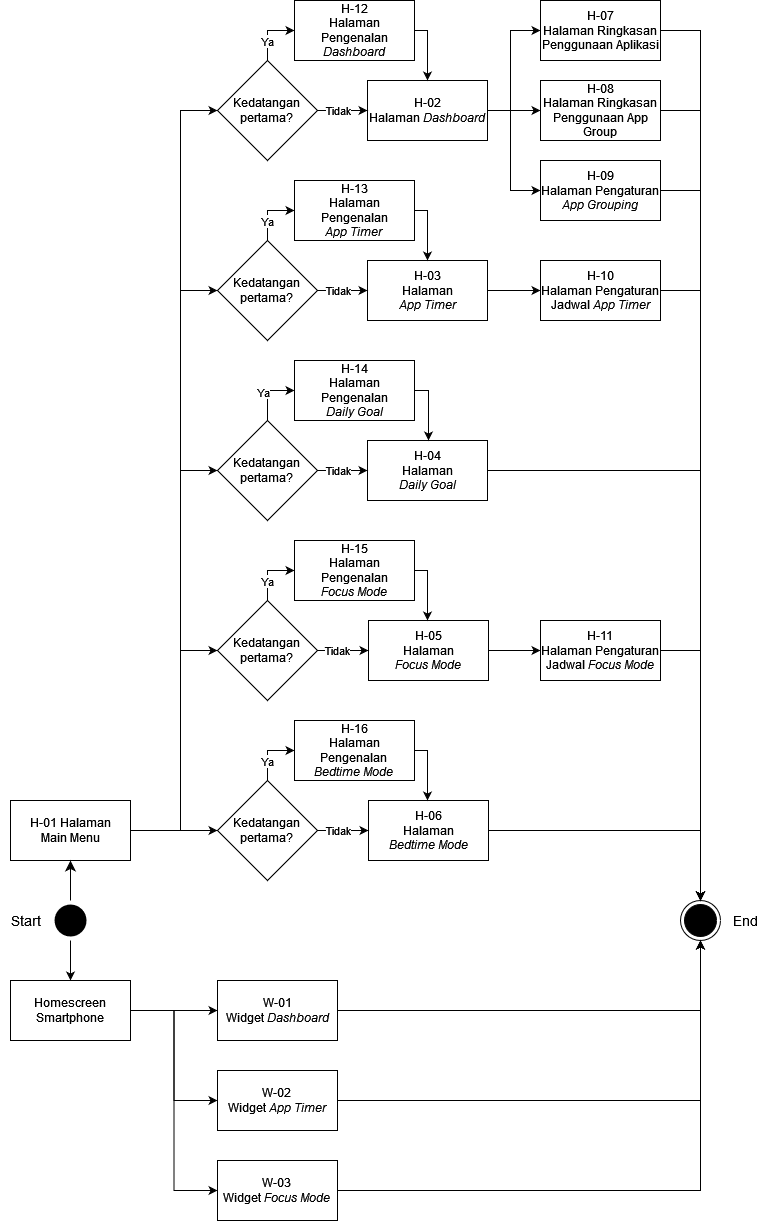
\includegraphics[width=0.68\textwidth]{chapter-3-diagram_user_flow.png}
  \caption{Diagram \textit{User Flow}}
  \label{fig:diagram_user_flow}
\end{figure}
\FloatBarrier

Pengguna dapat memulai \textit{user flow} dari halaman Main Menu, di mana pengguna akan disambut dengan deretan menu menuju 5 halaman utama. Di sini, \textit{user flow} bercabang ke tiap halaman fitur utama, jika pengguna pertama kali masuk ke halaman tersebut maka akan disambut dengan halaman pengenalan tentang fitur yang berkaitan. Berikut adalah penjelasan singkat tentang setiap cabang utama \textit{user flow}

\begin{enumerate}
  \item Saat masuk ke halaman Dashboard, pengguna dapat melihat data penggunaan \textit{smartphone}-nya. Kemudian pengguna dapat melihat detail penggunaan per aplikasi, untuk \textit{app group}, atau menambah \textit{app group} baru
  \item Saat masuk ke halaman \textit{App Timer}, pengguna dapat melihat daftar aplikasi yang telah dipasangi \textit{App Timer} jika ada. Pengguna juga dapat memasang \textit{App Timer} baru untuk aplikasi lain dengan memilihnya dari daftar aplikasi, di mana pengguna akan masuk ke Halaman Pengaturan Jadwal \textit{App Timer}.
  \item Saat masuk ke halaman \textit{Daily Goal}, pengguna dapat mengatur capaian utama apa yang ingin dijadikan target untuk hari tersebut. Pengguna juga dapat mengatur \textit{Daily Smartphone Evaluation} melalui halaman ini.
  \item Saat masuk ke halaman \textit{Focus Mode}, pengguna dapat melihat jadwal \textit{Focus Mode} yang sedang berlangsung, daftar jadwal \textit{Focus Mode} yang sudah dibuat, serta daftar aplikasi yang dinilai mendistraksi. Pengguna juga dapat mengatur aktivasi \textit{Focus Mode}, serta mengubah atau menambah jadwal \textit{Focus Mode} lewat Halaman Pengaturan Jadwal \textit{Focus Mode}, di mana pengguna juga dapat mengatur kembali aplikasi apa saja yang ingin diblokir selama jadwalnya aktif.
  \item Saat masuk ke halaman \textit{Bedtime Mode}, pengguna langsung dapat mengatur jadwal aktivasi dari \textit{Bedtime Mode}, serta mengatur perilaku dari \textit{Bedtime Mode} sendiri seperti aktivasi \textit{greyscale screen} atau \textit{Do Not Disturb}
\end{enumerate}

Selain Halaman Main Menu, \textit{user flow} juga dapat dimulai dari Homescreen \textit{smartphone}. Hal ini disebabkan karena widget adalah bagian dari aplikasi yang hanya dapat diakses dari Homescreen \textit{smartphone}. Widget bertujuan untuk memberikan fungsionalitas atau data dari aplikasi secara lebih cepat dengan tampilan yang lebih sederhana, tanpa memerlukan pengguna untuk mengakses aplikasinya. Maka dari itu, \textit{user flow} untuk widget langsung berakhir di widget tersebut.

% \subsection{Analisis Perbandingan Aplikasi}
% \label{subsec:analisis_user_flow}

% $ Kalau perlu split tabel prinsip desain
% \RaggedLeft
% \begin{footnotesize}
% \begin{longtable}[c]{|W{c}{0.07\textwidth}|>{\ccnormspacingcenter}m{0.18\textwidth}|>{\ccnormspacing}m{0.65\textwidth}|}
%   \caption{Daftar Penggunaan Prinsip Desain}
%   \label{tab:prinsip_desain} \\
%   \hline \rowcolor[HTML]{A3E5F5}
%   \multicolumn{1}{|c|}{\textbf{ID}} & \multicolumn{1}{|c|}{\textbf{Prinsip Desain}} & \multicolumn{1}{|c|}{\textbf{Penggunaan}} \\ \hline \endfirsthead
%   \hline \rowcolor[HTML]{A3E5F5}
%   \multicolumn{1}{|c|}{\textbf{ID}} & \multicolumn{1}{|c|}{\textbf{Prinsip Desain}} & \multicolumn{1}{|c|}{\textbf{Penggunaan}} \\ \hline \endhead

%   \hline \endfoot
  
%   \rowcolor[HTML]{DCF3FC} \multicolumn{3}{|l|}{\textbf{Prinsip Desain Digital Wellbeing}} \\ \hline
%   DP-01 & \textit{Empowerment} & Membuat pengaturan \textit{default} pada fitur dengan batas waktu dengan cara menyesuaikan pada kebiasaan pengguna \\ \hline
%   DP-02 & \textit{Awareness} & Meletakan data penggunaan \textit{smartphone} pengguna sebagai tampilan utama teratas dari aplikasi \\ \hline
%   DP-03 & \textit{Control} & Memberikan pengguna fleksibilitas dalam mengatur kemampuan penjadwalan fitur-fitur beserta deskripsi jelas \\ \hline
%   DP-04 & \textit{Adaptability} & Memberikan pengingat terhadap fitur-fitur yang telah dipasang pengguna sesuai dengan aplikasi yang sedang digunakan \\ \hline
% \end{longtable}
% \end{footnotesize}
% \justifying
% \FloatBarrier

% \RaggedLeft
% \begin{footnotesize}
% \begin{longtable}[c]{|W{c}{0.07\textwidth}|>{\ccnormspacingcenter}m{0.18\textwidth}|>{\ccnormspacing}m{0.65\textwidth}|}
%   \hline \rowcolor[HTML]{A3E5F5}
%   \multicolumn{1}{|c|}{\textbf{ID}} & \multicolumn{1}{|c|}{\textbf{Prinsip Desain}} & \multicolumn{1}{|c|}{\textbf{Penggunaan}} \\ \hline \endfirsthead
%   \hline \rowcolor[HTML]{A3E5F5}
%   \multicolumn{1}{|c|}{\textbf{ID}} & \multicolumn{1}{|c|}{\textbf{Prinsip Desain}} & \multicolumn{1}{|c|}{\textbf{Penggunaan}} \\ \hline \endhead

%   \hline \endfoot
  
%   \rowcolor[HTML]{DCF3FC} \multicolumn{3}{|l|}{\textbf{Prinsip Desain Interaksi}} \\ \hline
%   DP-05 & \textit{Visibility} & Membuat pembagian lokasi antarfitur yang jelas \\ \hline
%   DP-06 & \textit{Feedback} & Memberikan umpan balik yang sesuai saat pengguna melakukan aksi \\ \hline
%   DP-07 & \textit{Constraints} & Menonaktifkan tombol dari fitur yang tidak dapat diinteraksi tanpa menghapusnya \\ \hline
%   DP-08 & \textit{Consistency} & Konsistensi antara tampilan fitur pada halaman aplikasi dan widget \\ \hline
%   DP-09 & \textit{Affordance} & Desain yang jelas untuk elemen-elemen yang dapat diinteraksi \\ \hline

% \end{longtable}
% \end{footnotesize}
% \justifying
% \FloatBarrier

% $ Kalau perlu fungsionalitas 
% Keterkaitan Fungsionalitas mendahulukan fungsionalitas dari aplikasi Digital Wellbeing melihat terdapat beberapa fungsionalitas umum yang telah terdapat di aplikasi.

% $ Kalau ga perlu fungsionalitas

% \RaggedLeft
% \begin{footnotesize}
% \begin{longtable}[c]{|W{c}{0.06\textwidth}|>{\ccnormspacingcenter}m{0.15\textwidth}|>{\ccnormspacing}m{0.35\textwidth}|>{\ccnormspacingcenter}m{0.12\textwidth}|>{\ccnormspacingcenter}m{0.16\textwidth}|}
%   \caption{Daftar Fitur Prototipe Aplikasi}
%   \label{tab:daftar_fitur} \\
%   \hline \rowcolor[HTML]{A3E5F5}
%   \textbf{ID} & \textbf{Fitur} & \centering\textbf{Penjelasan} & \textbf{Tipe Fitur} & \textbf{Keterkaitan} \\ \hline \endfirsthead
%   \hline \rowcolor[HTML]{A3E5F5}
%   \textbf{ID} & \textbf{Fitur} & \centering\textbf{Penjelasan} & \textbf{Tipe Fitur} & \textbf{Keterkaitan} \\ \hline \endhead
%   \hline \endfoot

%   F-01 & \textit{Usage tracker} & Melacak penggunaan \textit{smartphone} dan aplikasi-aplikasi dari sisi lama penggunaan, jumlah pembukaan, dan notifikasi yang diterima & Sudah ada & UN-04, UG-03 \\ \hline
%   F-02 & \textit{Pie chart} & Menampilkan laporan data penggunaan \textit{smartphone} dan aplikasi-aplikasi untuk hari yang sedang berlangsung & Sudah ada & UN-04, UG-03 \\ \hline
%   F-03 & \textit{Bar chart} & Menampilkan ringkasan laporan data penggunaan \textit{smartphone} dan aplikasi-aplikasi & Sudah ada & UN-04, UG-03 \\ \hline
%   F-04 & \textit{Date range selector} & Memilih rentang tanggal untuk tampilan laporan penggunaan & Baru & UN-04, UG-03 \\ \hline
%   F-05 & \textit{Usage Summary} & Menampilkan ringkasan singkat tentang laporan penggunaan \textit{smartphone} dan aplikasi & Baru & UN-04, UG-03 \\ \hline
%   F-06 & Rekomendasi Aksi & Memberikan rekomendasi berdasarkan perilaku dari pengguna tentang aksi yang dapat dilakukan untuk memperbaiki kebiasaan digital pengguna & Baru & UN-03, UG-03 \\ \hline
%   F-07 & \textit{App Timer} & Membatasi waktu penggunaan aplikasi harian & Modifikasi & UG-02 \\ \hline
%   F-08 & Daftar aplikasi & Menampilkan seluruh aplikasi yang terdapat di \textit{smartphone} untuk diberikan aksi lanjutan sesuai konteks fitur & Sudah ada & UN-01 \\ \hline
%   F-09 & \textit{Search bar} & Mencari aplikasi yang terdapat pada daftar & Baru & UN-01 \\ \hline
%   F-10 & \textit{App group} & Mengelompokkan aplikasi-aplikasi berdasarkan kategori yang ditentukan pengguna & Baru & UN-01 \\ \hline
%   F-11 & \textit{Focus Mode} & Memblokir akses aplikasi dan informasi yang diberikan oleh aplikasi pilihan untuk waktu yang ditentukan atau sehari penuh & Modifikasi & UG-01, UG-02  \\ \hline
%   F-12 & \textit{Take a break} & Menunda pemblokiran dari fitur-fitur untuk waktu yang ditentukan & Modifikasi & UN-06, UG-06 \\ \hline
%   F-13 & \textit{Turn off for now} & Mematikan pemblokiran dari fitur-fitur untuk sehari penuh & Modifikasi & UN-06, UG-06 \\ \hline
%   F-14 & \textit{Bedtime Mode} & Mengubah \textit{smartphone} ke dalam perilaku mode tidur pada jadwal yang ditentukan & Sudah ada & UG-05 \\ \hline
%   F-15 & \textit{Greyscale screen} & Mengubah warna layar \textit{smartphone} menjadi hitam-putih & Sudah ada & UG-01 \\ \hline
%   F-16 & \textit{Do Not Disturb} & Mengalihkan pengguna ke layar pengaturan \textit{Do Not Disturb} bawaan \textit{smartphone} & Sudah ada & UG-01 \\ \hline
%   F-17 & Pengaturan notifikasi & Mengatur notifikasi terkait fitur atau aplikasi & Modifikasi & UG-01 \\ \hline
%   F-18 & Daftar Jadwal Aktivasi & Memberikan pengguna kemampuan untuk mengatur 0 atau lebih jadwal aktivasi fitur & Modifikasi & UN-05 \\ \hline
%   F-19 & \textit{Daily Goal} & Menentukan target harian dalam bentuk pesan yang dapat ditentukan pengguna untuk menjadi pengingat & Baru & UN-07, UG-04 \\ \hline
%   F-20 & \textit{Smartphone Usage Evaluation} & Memberikan notifikasi berisi evaluasi penggunaan \textit{smartphone} harian dan evaluasi untuk Daily Goal & Baru & UN-03, UN-09, UG-03 \\ \hline
%   F-21 & Deskripsi Fitur & Menjelaskan kegunaan dan tujuan dari sebuah fitur atau halaman fitur & Modifikasi & UN-03, UN-09, UG-03 \\ \hline

% \end{longtable}
% \end{footnotesize}
% \justifying
% \FloatBarrier

% $ Kalau perlu fungsionalitas

% \RaggedLeft
% \begin{footnotesize}
  
% \begin{longtable}[c]{|W{c}{0.05\textwidth}|>{\ccnormspacingcenter}m{0.14\textwidth}|>{\ccnormspacing}m{0.2\textwidth}|>{\ccnormspacingcenter}m{0.12\textwidth}|>{\ccnormspacingcenter}m{0.14\textwidth}|>{\ccnormspacingcenter}m{0.16\textwidth}|}
%   \caption{Daftar Fitur Prototipe Aplikasi}
%   \label{tab:daftar_fitur} \\
%   \hline \rowcolor[HTML]{A3E5F5}
%   \textbf{ID} & \textbf{Fitur} & \centering\textbf{Penjelasan} & \textbf{Tipe Fitur} & \textbf{Keterkaitan Kebutuhan \& Tujuan} & \textbf{Keterkaitan Fungsionalitas} \\ \hline \endfirsthead
%   \hline \rowcolor[HTML]{A3E5F5}
%   \textbf{ID} & \textbf{Fitur} & \centering\textbf{Penjelasan} & \textbf{Tipe Fitur} & \textbf{Keterkaitan Kebutuhan \& Tujuan} & \textbf{Keterkaitan Fungsionalitas} \\ \hline \endhead
%   \hline \endfoot

%   F-01 & \textit{Usage tracker} & Melacak penggunaan \textit{smartphone} dan aplikasi-aplikasi dari sisi lama penggunaan, jumlah pembukaan, dan notifikasi yang diterima & Sudah ada & UN-04, UG-03 & FD-01, FD-02 \\ \hline
%   F-02 & \textit{Pie chart} & Menampilkan laporan data penggunaan \textit{smartphone} dan aplikasi-aplikasi untuk hari yang sedang berlangsung & Sudah ada & UN-04, UG-03 & FD-03 \\ \hline
%   F-03 & \textit{Bar chart} & Menampilkan ringkasan laporan data penggunaan \textit{smartphone} dan aplikasi-aplikasi & Modifikasi & UN-04, UG-03 & FD-03 \\ \hline
%   F-04 & \textit{Date range selector} & Memilih rentang tanggal untuk tampilan laporan penggunaan & Baru & UN-04, UG-03 & FU-03 \\ \hline
%   F-05 & \textit{Usage Summary} & Menampilkan ringkasan singkat tentang laporan penggunaan \textit{smartphone} dan aplikasi & Baru & UN-04, UG-03 & FU-03 \\ \hline
%   F-06 & Rekomendasi Aksi & Memberikan rekomendasi berdasarkan perilaku dari pengguna tentang aksi yang dapat dilakukan untuk memperbaiki kebiasaan digital pengguna & Baru & UN-03, UG-03 & - \\ \hline
%   F-07 & \textit{App Timer} & Membatasi waktu penggunaan aplikasi harian & Sudah ada & UG-02 & FD-05 \\ \hline
%   F-08 & Daftar aplikasi & Menampilkan seluruh aplikasi yang terdapat di \textit{smartphone} untuk diberikan aksi lanjutan sesuai konteks fitur & Sudah ada & UN-01 & FD-04 \\ \hline
%   F-09 & \textit{Search bar} & Mencari aplikasi yang terdapat pada daftar & Baru & UN-01 & - \\ \hline
%   F-10 & \textit{App group} & Mengelompokkan aplikasi-aplikasi berdasarkan kategori yang ditentukan pengguna & Baru & UN-01 & - \\ \hline
%   F-11 & \textit{Focus Mode} & Memblokir akses aplikasi dan informasi yang diberikan oleh aplikasi  pilihan untuk waktu yang ditentukan atau sehari penuh & Modifikasi & UG-01, UG-02 & FD-08, FD-09 \\ \hline
%   F-12 & \textit{Take a break} & Menunda pemblokiran dari fitur-fitur untuk waktu yang ditentukan & Modifikasi & UN-06, UG-06 & FD-11 \\ \hline
%   F-13 & \textit{Turn off for now} & Mematikan pemblokiran dari fitur-fitur untuk sehari penuh & Modifikasi & UN-06, UG-06 & FD-11 \\ \hline
%   F-14 & \textit{Bedtime Mode} & Mengubah \textit{smartphone} ke dalam perilaku mode tidur pada jadwal yang ditentukan & Modifikasi & UG-05 & FD-12 \\ \hline
%   F-15 & \textit{Greyscale screen} & Mengubah warna layar \textit{smartphone} menjadi hitam-putih & Sudah ada & UG-01 & FD-15 \\ \hline
%   F-16 & \textit{Do Not Disturb} & Mengalihkan pengguna ke layar pengaturan Do Not Disturb bawaan \textit{smartphone} & Sudah ada & UG-01 & - \\ \hline
%   F-17 & Pengaturan notifikasi & Mengatur notifikasi terkait fitur atau aplikasi & Modifikasi & UG-01 & - \\ \hline
%   F-18 & Daftar Jadwal Aktivasi & Memberikan pengguna kemampuan untuk mengatur 0 atau lebih jadwal aktivasi fitur & Modifikasi & UN-05 & FD-10 \\ \hline
%   F-19 & \textit{Daily Goal} & Menentukan target harian dalam bentuk pesan yang dapat ditentukan pengguna untuk menjadi pengingat & Baru & UN-07, UG-04 & FU-13 \\ \hline
%   F-20 & \textit{Smartphone Usage Evaluation} & Memberikan notifikasi berisi evaluasi penggunaan \textit{smartphone} harian dan evaluasi untuk Daily Goal & Baru & UN-03, UN-09, UG-03 & FU-07 \\ \hline
%   F-21 & \textit{Deskripsi Fitur} & Menjelaskan kegunaan dan tujuan dari sebuah fitur atau halaman fitur & Sudah ada & UN-03, UN-09, UG-03 & FD-16 \\ \hline

% \end{longtable}
% \end{footnotesize}
% \justifying

% $ Kalau perlu fungsionalitas dan landscape
% \newpage
% \begin{landscape}
%   \RaggedLeft
%   \begin{footnotesize}
% \begin{longtable}[c]{|W{c}{0.06\textwidth}|>{\ccnormspacingcenter}m{0.15\textwidth}|>{\ccnormspacing}m{0.9\textwidth}|>{\ccnormspacingcenter}m{0.12\textwidth}|>{\ccnormspacingcenter}m{0.18\textwidth}|>{\ccnormspacingcenter}m{0.18\textwidth}|}
%   \caption{Daftar Fitur Prototipe Aplikasi}
%   \label{tab:daftar_fitur} \\
%   \hline \rowcolor[HTML]{A3E5F5}
%   \textbf{ID} & \textbf{Fitur} & \centering\textbf{Penjelasan} & \textbf{Tipe Fitur} & \textbf{Keterkaitan Kebutuhan \& Tujuan} & \textbf{Keterkaitan Fungsionalitas} \\ \hline \endfirsthead
%   \hline \rowcolor[HTML]{A3E5F5}
%   \textbf{ID} & \textbf{Fitur} & \centering\textbf{Penjelasan} & \textbf{Tipe Fitur} & \textbf{Keterkaitan Kebutuhan \& Tujuan} & \textbf{Keterkaitan Fungsionalitas} \\ \hline \endhead
%   \hline \endfoot

%   F-01 & \textit{Usage tracker} & Melacak penggunaan \textit{smartphone} dan aplikasi-aplikasi dari sisi lama penggunaan, jumlah pembukaan, dan notifikasi yang diterima & Sudah ada & UN-04, UG-03 & FD-01, FD-02 \\ \hline
%   F-02 & \textit{Pie chart} & Menampilkan laporan data penggunaan \textit{smartphone} dan aplikasi-aplikasi untuk hari yang sedang berlangsung & Sudah ada & UN-04, UG-03 & FD-03 \\ \hline
%   F-03 & \textit{Bar chart} & Menampilkan ringkasan laporan data penggunaan \textit{smartphone} dan aplikasi-aplikasi & Modifikasi & UN-04, UG-03 & FD-03 \\ \hline
%   F-04 & \textit{Date range selector} & Memilih rentang tanggal untuk tampilan laporan penggunaan & Baru & UN-04, UG-03 & FU-03 \\ \hline
%   F-05 & \textit{Usage Summary} & Menampilkan ringkasan singkat tentang laporan penggunaan \textit{smartphone} dan aplikasi & Baru & UN-04, UG-03 & FU-03 \\ \hline
%   F-06 & Rekomendasi Aksi & Memberikan rekomendasi berdasarkan perilaku dari pengguna tentang aksi yang dapat dilakukan untuk memperbaiki kebiasaan digital pengguna & Baru & UN-03, UG-03 & - \\ \hline
%   F-07 & \textit{Dashboard Widget} & Menampilkan laporan penggunaan \textit{smartphone} dan aplikasi untuk hari yang sedang berlangsung & Modifikasi & UN-02, UG-03 & FD-03, FD-04 \\ \hline
%   F-08 & \textit{App Timer} & Membatasi waktu penggunaan aplikasi harian & Sudah ada & UG-02 & FD-05 \\ \hline
%   F-09 & \textit{App Timer Widget}  & Menampilkan daftar sisa waktu penggunaan aplikasi yang dipasang App Timer & Baru & UN-02, UG-02 & FU-06 \\ \hline
%   F-10 & Daftar aplikasi & Menampilkan seluruh aplikasi yang terdapat di \textit{smartphone} untuk diberikan aksi lanjutan sesuai konteks fitur & Sudah ada & UN-01 & FD-04 \\ \hline
%   F-11 & \textit{Search bar} & Mencari aplikasi yang terdapat pada daftar & Baru & UN-01 & - \\ \hline
%   F-12 & \textit{App group} & Mengelompokkan aplikasi-aplikasi berdasarkan kategori yang ditentukan pengguna & Baru & UN-01 & - \\ \hline
%   F-13 & \textit{Focus Mode} & Memblokir akses aplikasi dan informasi yang diberikan oleh aplikasi  pilihan untuk waktu yang ditentukan atau sehari penuh & Modifikasi & UG-01, UG-02 & FD-08, FD-09 \\ \hline
%   F-14 & \textit{Take a break} & Menunda pemblokiran dari fitur-fitur untuk waktu yang ditentukan & Modifikasi & UN-06, UG-06 & FD-11 \\ \hline
%   F-15 & \textit{Turn off for now} & Mematikan pemblokiran dari fitur-fitur untuk sehari penuh & Modifikasi & UN-06, UG-06 & FD-11 \\ \hline
%   F-16 & \textit{Focus Mode Widget} & Menampilkan jadwal aktivasi Focus Mode dan fungsionalitas aktivasi dari fitur Focus Mode & Baru & UN-02, UG-01 & FU-06 \\ \hline
%   F-17 & \textit{Bedtime Mode} & Mengubah \textit{smartphone} ke dalam perilaku mode tidur pada jadwal yang ditentukan & Modifikasi & UG-05 & FD-12 \\ \hline
%   F-18 & \textit{Greyscale screen} & Mengubah warna layar \textit{smartphone} menjadi hitam-putih & Sudah ada & UG-01 & FD-15 \\ \hline
%   F-19 & \textit{Do Not Disturb} & Mengalihkan pengguna ke layar pengaturan Do Not Disturb bawaan \textit{smartphone} & Sudah ada & UG-01 & - \\ \hline
%   F-20 & Pengaturan notifikasi & Mengatur notifikasi terkait fitur atau aplikasi & Modifikasi & UG-01 & - \\ \hline
%   F-21 & Daftar Jadwal Aktivasi & Memberikan pengguna kemampuan untuk mengatur 0 atau lebih jadwal aktivasi fitur & Modifikasi & UN-05 & FD-10 \\ \hline
%   F-22 & \textit{Daily Goal} & Menentukan target harian dalam bentuk pesan yang dapat ditentukan pengguna untuk menjadi pengingat & Baru & UN-07, UG-04 & FU-13 \\ \hline
%   F-23 & \textit{Smartphone Usage Evaluation} & Memberikan notifikasi berisi evaluasi penggunaan \textit{smartphone} harian dan evaluasi untuk Daily Goal & Baru & UN-03, UN-09, UG-03 & FU-07 \\ \hline
%   F-24 & \textit{Deskripsi Fitur} & Menjelaskan kegunaan dan tujuan dari sebuah fitur atau halaman fitur & Sudah ada & UN-03, UN-09, UG-03 & FD-16 \\ \hline


% \end{longtable}
% \end{footnotesize}
% \justifying
% \FloatBarrier

% \end{landscape}

% $ Kalau perlu fungsionalitas, goals, dan landscape

% \begin{landscape}
% \RaggedLeft
% \begin{footnotesize}

% \begin{longtable}[c]{|W{c}{0.06\textwidth}|>{\ccnormspacingcenter}m{0.2\textwidth}|>{\ccnormspacing}m{0.65\textwidth}|>{\ccnormspacingcenter}m{0.12\textwidth}|>{\ccnormspacingcenter}m{0.17\textwidth}|>{\ccnormspacingcenter}m{0.17\textwidth}|>{\ccnormspacingcenter}m{0.15\textwidth}|}
%   \caption{Daftar Fitur Prototipe Aplikasi}
%   \label{tab:daftar_fitur} \\
%   \hline \rowcolor[HTML]{A3E5F5}
%   \textbf{ID} & \textbf{Fitur} & \centering\textbf{Penjelasan} & \textbf{Tipe Fitur} & \textbf{Keterkaitan Kebutuhan \& Tujuan} & \textbf{Keterkaitan Fungsionalitas} & \textbf{Keterkaitan \textit{Goals}} \\ \hline \endfirsthead
%   \hline \rowcolor[HTML]{A3E5F5}
%   \textbf{ID} & \textbf{Fitur} & \centering\textbf{Penjelasan} & \textbf{Tipe Fitur} & \textbf{Keterkaitan Kebutuhan \& Tujuan} & \textbf{Keterkaitan Fungsionalitas} & \textbf{Keterkaitan \textit{Goals}} \\ \hline \endhead
%   \hline \endfoot

%   F-01 & \textit{Usage tracker} & Melacak penggunaan \textit{smartphone} dan aplikasi-aplikasi dari sisi lama penggunaan, jumlah pembukaan, dan notifikasi yang diterima & Sudah ada & UN-04, UG-03 & FD-01, FD-02 & G-03 \\ \hline
%   F-02 & \textit{Pie chart} & Menampilkan laporan data penggunaan \textit{smartphone} dan aplikasi-aplikasi untuk hari yang sedang berlangsung & Sudah ada & UN-04, UG-03 & FD-03 & G-03 \\ \hline
%   F-03 & \textit{Bar chart} & Menampilkan ringkasan laporan data penggunaan \textit{smartphone} dan aplikasi-aplikasi & Modifikasi & UN-04, UG-03 & FD-03 & G-03 \\ \hline
%   F-04 & \textit{Date range selector} & Memilih rentang tanggal untuk tampilan laporan penggunaan & Baru & UN-04, UG-03 & FU-03 & G-01, G-03 \\ \hline
%   F-05 & \textit{Usage Summary} & Menampilkan ringkasan singkat tentang laporan penggunaan \textit{smartphone} dan aplikasi & Baru & UN-04, UG-03 & FU-03 & G-01, G-03 \\ \hline
%   F-06 & Rekomendasi Aksi & Memberikan rekomendasi berdasarkan perilaku dari pengguna tentang aksi yang dapat dilakukan untuk memperbaiki kebiasaan digital pengguna & Baru & UN-03, UG-03 & - & G-04 \\ \hline
%   F-07 & \textit{App Timer} & Membatasi waktu penggunaan aplikasi harian & Sudah ada & UG-02 & FD-05 & G-03 \\ \hline
%   F-08 & Daftar aplikasi & Menampilkan seluruh aplikasi yang terdapat di \textit{smartphone} untuk diberikan aksi lanjutan sesuai konteks fitur & Sudah ada & UN-01 & FD-04 & G-03 \\ \hline
%   F-09 & \textit{Search bar} & Mencari aplikasi yang terdapat pada daftar & Baru & UN-01 & - & G-01, G-03 \\ \hline
%   F-10 & \textit{App group} & Mengelompokkan aplikasi-aplikasi berdasarkan kategori yang ditentukan pengguna & Baru & UN-01 & - & G-01, G-03 \\ \hline
%   F-11 & \textit{Focus Mode} & Memblokir akses aplikasi dan informasi yang diberikan oleh aplikasi  pilihan untuk waktu yang ditentukan atau sehari penuh & Modifikasi & UG-01, UG-02 & FD-08, FD-09 & G-03 \\ \hline
%   F-12 & \textit{Take a break} & Menunda pemblokiran dari fitur-fitur untuk waktu yang ditentukan & Modifikasi & UN-06, UG-06 & FD-11 & G-03 \\ \hline
%   F-13 & \textit{Turn off for now} & Mematikan pemblokiran dari fitur-fitur untuk sehari penuh & Modifikasi & UN-06, UG-06 & FD-11 & G-03 \\ \hline
%   F-14 & \textit{Bedtime Mode} & Mengubah \textit{smartphone} ke dalam perilaku mode tidur pada jadwal yang ditentukan & Modifikasi & UG-05 & FD-12 & G-03 \\ \hline
%   F-15 & \textit{Greyscale screen} & Mengubah warna layar \textit{smartphone} menjadi hitam-putih & Sudah ada & UG-01 & FD-15 & G-03 \\ \hline
%   F-16 & \textit{Do Not Disturb} & Mengalihkan pengguna ke layar pengaturan Do Not Disturb bawaan \textit{smartphone} & Sudah ada & UG-01 & - & G-03 \\ \hline
%   F-17 & Pengaturan notifikasi & Mengatur notifikasi terkait fitur atau aplikasi & Modifikasi & UG-01 & - & G-03 \\ \hline
%   F-18 & Daftar Jadwal Aktivasi & Memberikan pengguna kemampuan untuk mengatur 0 atau lebih jadwal aktivasi fitur & Modifikasi & UN-05 & FD-10 & G-01, G-03 \\ \hline
%   F-19 & \textit{Daily Goal} & Menentukan target harian dalam bentuk pesan yang dapat ditentukan pengguna untuk menjadi pengingat & Baru & UN-07, UG-04 & FU-13 & G-04 \\ \hline
%   F-20 & \textit{Smartphone Usage Evaluation} & Memberikan notifikasi berisi evaluasi penggunaan \textit{smartphone} harian dan evaluasi untuk Daily Goal & Baru & UN-03, UN-09, UG-03 & FU-07 & G-04 \\ \hline
%   F-21 & \textit{Deskripsi Fitur} & Menjelaskan kegunaan dan tujuan dari sebuah fitur atau halaman fitur & Sudah ada & UN-03, UN-09, UG-03 & FD-16 & G-02, G-03 \\ \hline

% \end{longtable}
% \end{footnotesize}
% \justifying
% \end{landscape}
% \FloatBarrier

% \begin{enumerate}
%   \item Terdapat fitur-fitur dengan tampilan dan interaksi sederhana yang dirancang meningkatkan efisiensi (G-01) yang cukup besar bagi pengguna dalam melakukan kegiatannya. Fitur \textit{Date range selector} (F-04) dan \textit{Usage summary} (F-05) dapat mempermudah pengguna dalam mencari data penggunaan pada tanggal atau jangka waktu tertentu serta menganalisis ringkasan penggunaan. Adapun fitur \textit{Searchbar} (F-05) untuk mempermudah mencari aplikasi yang ingin dianalisis atau diblokir, dibandingkan dengan aplikasi Digital Wellbeing awalnya di mana pengguna harus \textit{scrolling} daftar yang panjang untuk mencari aplikasi tertentu.
  
%   \item Terdapat juga fitur-fitur yang memiliki kompleksitas lebih tinggi yang dirancang untuk membantu penggunanya juga melakukan pengaturan secara lebih efisien (G-01 dan G-03). Fitur \textit{App Group} (F-10) dirancang agar pengguna dapat memasang App Timer atau Focus Mode kepada beberapa aplikasi sekaligus, dibandingkan dengan aplikasi Digital Wellbeing awalnya di mana pengguna harus melakukan hal yang sama secara berkali-kali. Adapun \textit{daftar jadwal aktivasi} (F-18) yang ketika digabungkan dengan App Timer atau Focus Mode dapat mempermudah pengguna untuk mengatur jadwal aktivasi per harinya secara langsung, tanpa melakukan pengubahan setiap hari. Misalnya, jika pengguna ingin membatasi penggunaan suatu aplikasi sosial media selama 2 jam di hari biasa dan 4 jam di akhir pekan, pengguna dapat langsung mengatur App Timernya cukup sekali, di mana pada aplikasi Digital Wellbeing awalnya pengguna harus menyesuaikan App Timer di hari yang bersangkutan.
  
%   \item Kebutuhan akan deskripsi fitur (F-21) perlu ditekankan untuk memenuhi \textit{usability goals Learnability}, di mana adanya tambahan deskripsi untuk fitur-fitur dapat mempermudah pengguna baru untuk mempelajari dan menggunakannya. Deskripsi fitur dapat berbentuk tulisan, atau ilustrasi dengan gambar. Contoh deskripsi fitur dapat dilihat dengan lebih jelas pada saat implementasi prototipe \textit{low-fidelity} pada bagian \ref{subsec:lofi_implementasi}. 
  
%   \item Fitur seperti Rekomendasi Aksi (F-06), \textit{Daily Goal} (F-19), dan \textit{Smartphone Usage Evaluation} (F-20) dirancang untuk memenuhi \textit{user experience goal Motivating} (G-04), dengan memberikan pesan-pesan memotivasi, memberikan rekomendasi dalam bentuk tindakan yang dapat dilakukan untuk memperbaiki kebiasaan, atau memberikan pesan di akhir hari tentang berapa lama waktu penggunaan \textit{smartphone} yang berhasil dikurangi dibandingkan dengan hari kemarin.
% \end{enumerate}
